\documentclass[a4paper,12pt]{article}

% Import the deliverable package from common directory
\usepackage{../common/deliverable}

% Tell LaTeX where to find graphics files
\graphicspath{{../common/logos/}{./figures/}{../}}

\usepackage{xspace}
\usepackage{lipsum}
\usepackage{listings}
\usepackage{xcolor} % for custom colors
\usepackage[round]{natbib}

% Small font size in lstlistings
\lstset{basicstyle=\ttfamily\small}

% Define a custom DSL (keywords of your choice)
\lstdefinelanguage{TensorIR}{
    morekeywords={alloca,gemm,gemv,fuse,subview},
    morecomment=[l]{\;},
}

% Block comment
\newcommand{\mycomment}[1]{}

% Set the deliverable number (without the D prefix, it's added automatically)
\setdeliverableNumber{3.2}

% Begin document
\begin{document}

% Create the title page with the title as argument
\maketitlepage{Co-Design and Energy Efficiency Report I}

\newpage

% Main Table using the new environment and command
\begin{deliverableTable}
    \tableEntry{Deliverable title}{Co-Design and Energy Efficiency Report}
    \tableEntry{Deliverable number}{D3.2}
    \tableEntry{Deliverable version}{v1}
    \tableEntry{Date of delivery}{August 31, 2025}
    \tableEntry{Actual date of delivery}{August 29, 2025}
    \tableEntry{Nature of deliverable}{Report}
    \tableEntry{Dissemination level}{Public}
    \tableEntry{Work Package}{WP3}
    \tableEntry{Partner responsible}{BADW-LRZ}
\end{deliverableTable}

% Abstract and Keywords Section
\begin{deliverableTable}
    \tableEntry{Abstract}{\lipsum[1][1-5]}
    \tableEntry{Keywords}{performance; benchmarks; gpu-programming; Keyword 4; Keyword 5}
\end{deliverableTable}

\newpage

\begin{documentControl}
    \addVersion{0.1}{22/08/2025}{Ivan Pribec}{Initial draft}
    \addVersion{0.2}{25/08/2025}{Enes Mustafa Soydan}{Added results of RUB group}
    \addVersion{0.3}{29/08/2025}{Martin Kronbichler}{Review}
    \addVersion{1.0}{29/08/2025}{Ivan Pribec}{Final version}
\end{documentControl}

\subsection*{{Approval Details}}
Approved by: Martin Kronbichler \\
Approval Date: August 29, 2025

\subsection*{{Distribution List}}
\begin{itemize}
    \item [] - Project Coordinators (PCs)
    \item [] - Work Package Leaders (WPLs)
    \item [] - Steering Committee (SC)
    \item [] - European Commission (EC)
\end{itemize}

\vspace*{2cm}

\disclaimer

\newpage

\tableofcontents % Automatically generated and hyperlinked Table of Contents

\newpage

\section{{Introduction}}

\mycomment{
    % goals of the WP
    \begin{itemize}
        \item Investigate novel hardware and software solutions to leverage the latest advancements in high-performance computing
    to achieve optimal performance
        \item Identify and evaluate emerging technologies that can be exploited to enhance the capabilities of the exascale computing
    system.
        \item Explore and implement techniques to optimize energy consumption and power efficiency in the exascale computing
    infrastructure.
        \item Identify and address bottlenecks in the system to improve overall computational efficiency.
    \end{itemize}
}

This report describes our advances investigating novel hardware and software solutions, and evaluating emerging technologies for exascale computing with the final goal of achieving state-of-the-art performance and optimal technology exploitation.

Our main achievement in this period has been the preparation and analysis of benchmark kernels for the matrix-free application of discrete finite element operators, see also our overall frameworks described in \cite{Kronbichler12,Kronbichler19}, focused on addressing newer GPU architectures. 

The benchmark repository is made publically available at: \url{https://github.com/dealii-X/benchmarks/}

The preparation of these benchmarks has been the focus of Milestone \#3 -- Public repository of benchmark sets for performance evaluation -- verified by means of runs of the software on at
least three different accelerated platforms.

For performance optimization purposes we have focused on two families of kernels, the CEED\footnote{Center for Efficient Exascale Discretization, Exascale Computing Project, \url{https://ceed.exascaleproject.org/}} Bakeoff Problems\footnote{\url{https://libceed.org/en/latest/examples/bps/}} and Streaming Kernels, that serve as a suitable proxy for the algorithmic core of simulation codes using high-order finite elements.



The CEED Bakeoff Problems~\citep{Fischer20scalability} are a benchmark to measure the evaluation speed of the basic finite element operators (discretized bilinear forms), posed for problems on hexahedral grids, and the primary focus being sum factorization techniques. 
Both scalar and vector  problems are included in the benchmarks. So far our efforts have been focused on the scalar problems.
Each of the Bakeoff Problems (BP) has an associated Benchmark Kernel (BK) that evaluates a particular 
finite element operator and is of high arithmetic intensity. 
The efficient implementation of these kernels is paramount to obtain good performance. 

The benchmark kernels are based on a numerical quadrature approach to evaluate the finite-element integrals and exploit algebraic sum factorization techniques \citep{Deville02} to achieve an affordable evaluation of high-order finite element operators in comparison to the naive nested sum algorithm or dense interpolation matrices. This type of technique has been popularized in recent years by several groups, including the deal.II authors~\citep{Kronbichler12,Kronbichler19,Arndt21}. The translation of these techniques to modern GPU architectures, see also the work by~\cite{Swirydowicz19}, remains an open challenge at both software and hardware level due to the heterogeneity of both devices (CPUs, GPUs and other accelerators) and parallel programming frameworks provided by different vendors.

The Streaming Kernels \citep[Table 1]{chalmers20} capture a second group of low intensity operations, where memory movement is dominant.
The kernels generally take one or two long vectors as arguments. 
The first four kernels included are: copy (COPY), scaled sum of vectors (AXPBY), squared norm (NRM2), and inner product of two vectors (DOT). 
The fifth kernel is the fused conjugate gradient update that involves the combination of a scaled sum and norm of a residual vector in a single sweep.    
The last two kernels are the gather and scatter kernels that involve packing and unpacking the degrees of freedom associated with a given finite element mesh into a linear vector.
The gather and scatter kernels are tied to a particular mesh and finite element space, requiring more extensive driver setup. 
Hence, they are not addressed in this report.

\begin{itemize}
\item CUDA Support: Enabling programming support for NVIDIA GPUs using the CUDA parallel computing model and
supporting compatibility with AMDs HIP framework.
\item SYCL Integration: Incorporating SYCL (Standard C++ for heterogeneous computing) for programming heterogeneous
systems using C++. Porting from and compatibility with CUDA.
\item Using OpenMP and/or OpenACC offloading techniques and ensuring their compatibility on different
platforms.
\item Employing parallel programming techniques like SIMD (Single Instruction, Multiple Data) for efficient accelerator
and CPU utilization.
\item We will support programming approaches and frameworks such as Kokkos (already supported by deal.II) and RAJA
that supporting a range of accelerator programming paradigms ensure flexibility and compatibility with different
hardware architectures, enabling developers to harness the full potential of accelerators in their applications. This avoids maintaining paradigm-specific code branches in parallel.
\end{itemize}

\newpage

\section{CEED Bakeoff Problems}

To study the performance and portability of high-order finite element implementation we focus on a subset of the CEED Bakeoff problems, designed to test and compare
the performance of high-order codes.

The subset we have focused on so far are,
\begin{itemize}
    \item BK1: scalar PCG with mass matrix, $q = p+2$
    \item BK3: scalar PCG with stiffness matrix, $q = p+1$
    \item BK5: scalar PCG with stiffness matrix, $q = p+2$
\end{itemize}
The benchmarks kernels form the algorithm core of the benchmark problems (BP), which include a complete finite element workflow, including mesh setup, partitioning, and parallel computation.

The initial kernels have been implemented in three variants: 1) sequential kernels for verification, 2) using Kokkos Core, a C++ programming model for writing portable applications, part of the larger Kokkos C++ Performance Portability Programming Ecosystem\footnote{Kokkos, \url{https://kokkos.org}} and 3) using the CUDA Driver API. In order to evaluate the impact of parallelization strategies, the Kokkos and CUDA-based kernels have several sub-variants that use different thread-mapping strategies, i.e. the assignment of degrees-of-freedom and quadrature points to GPU threads.

In order to obtain a wider impression of GPU programming models available we have also created variants using OpenCL, OpenMP target offloading and variant for the Tiny Tensor Compiler, a recently introduced domain specific language for tensor operations from Intel. 

In the following sub-sections we describe our preliminary findings from the BK1 benchmark.
We present experiments from multiple accelerator devices, showcasing their throughput capabilities in terms of degrees of freedom updated per second versus the problem size.
The problem size is measured in number of degrees of freedom (DoFs) which is related closely to the number of elements.
Besides the variation w.r.t. problem size, we also study the influence of the quadrature order.

In the experiments presented below, the following compilers (including OpenMP) are used:
\begin{itemize}
    \item Intel oneAPI Toolkit version 2024.1 (`icpx')
    \item Nvidia HPC SDK v2024.5 (`nvc++')
    \item Tiny Tensor Compiler v0.3.1
\end{itemize}
The libraries used are
\begin{itemize}
    \item Kokkos Version 4.6.2
    \item Intel OpenCL (driver version: )
    \item Nvidia OpenCL (driver version: )
\end{itemize}

\subsection{Kokkos and CUDA Performance Results}
{\bf BK1.} Early performance results for the different test cases are shown in Figure~\ref{fig:BK1_1} and Figure~\ref{fig:BK1_2}, evaluated on an Nvidia H100 GPU. Each test case uses 3D thread blocks, determines the number of quadrature points at run time, and employs thread blocks for element-wise computations. The only difference between the two cases is the programming model: Figure 1 presents the results obtained with CUDA, while Figure 2 shows those from the Kokkos library.
The first finding is that polynomial order 1 shows lower performance compared to higher-order elements in both test cases. This behavior, rooted in a first-order polynomial, is configured with 27 threads per block. This leads to under-utilization of the warp (size 32) on the target hardware.
The second finding is that Kokkos achieves approximately 90\% of the performance observed with the CUDA model, demonstrating that the performance portability model introduces only a minor overhead.

\begin{figure}
\centering
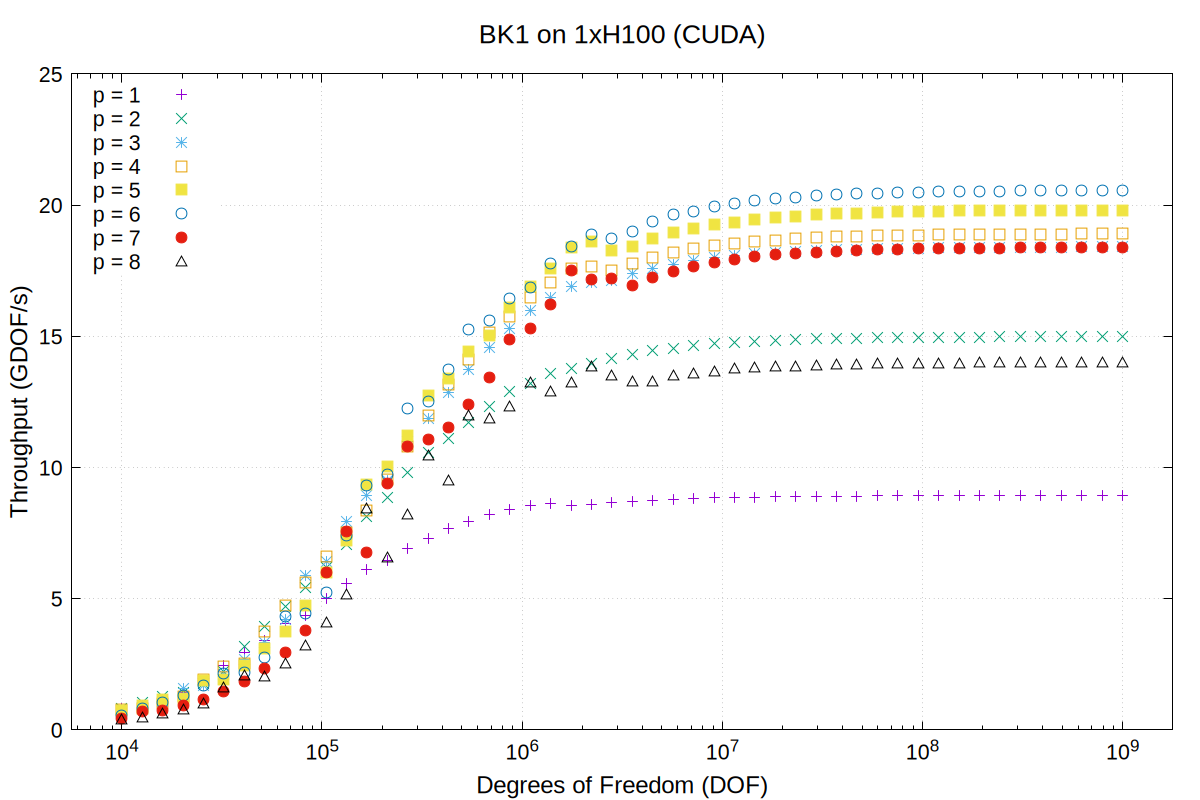
\includegraphics[width=0.8\textwidth]{BK1_1}
\caption{BK1 performance results on Nvidia H100 GPU with CUDA programming model. Various polynomial orders are tested, and saturation of hardware resources is visible after $10^6$ degrees of freedom. Polynomial order 1 performs the worst due to under-occupation of the single warp.}
\label{fig:BK1_1}
\end{figure}
\begin{figure}
\centering
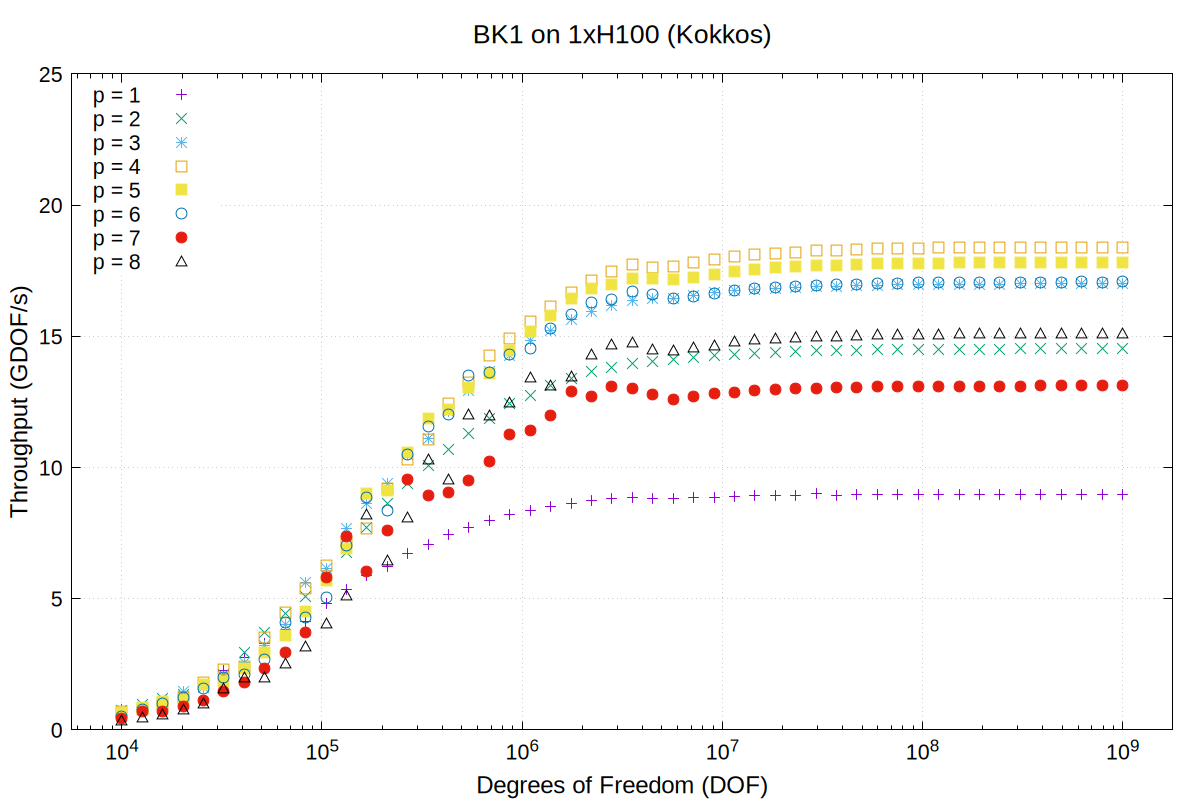
\includegraphics[width=0.8\textwidth]{BK1_2}
\caption{BK1 performance results on an NVIDIA H100 GPU using the Kokkos library. The same test conditions and optimization techniques as in Figure 1 were applied. Kokkos attains nearly 90\% of the performance delivered by CUDA.}
\label{fig:BK1_2}
\end{figure}

{\bf BK5.} Unlike the multiple polynomial order evaluations in the BK1 test cases, we analyzed the kernels with a fixed cubic polynomial order (p=3) and templated quadrature points. Using templates shifts certain computations from runtime to compile-time, allowing the compiler to apply optimizations. As a result, templated implementations are often significantly faster, in most cases improving performance by 30\% at least, compared to their runtime counterparts.

Both CUDA and Kokkos kernels were implemented with three-dimensional thread blocks and a simple data mapping approach, where each thread operates on a single data entry. The total number of degrees of freedom (DOF) in this test case is 27 million. Kernel performance values were measured by NVIDIA Nsight Compute. In these measurements, both CUDA and Kokkos executions completed in 0.71 ms, showing identical performance. Nsight Compute reported an arithmetic intensity of 1.97 FLOP/byte, which places these kernels in the memory-bound region of the roofline model for the H100 GPU. The achieved performance was 5.7 TFLOPs, compared to the hardware limit of 6.6 TFLOPs at this arithmetic intensity. This corresponds to 86\% of peak bandwidth utilization (2.88 TB/s out of 3.2 TB/s). The kernels also achieved 75\% occupancy, and register usage per thread was identified as the primary limiting factor.

Overall, the results demonstrate that both CUDA and Kokkos BK5 implementations deliver near-optimal performance on the H100, efficiently exploiting available memory bandwidth and achieving performance levels very close to the hardware limits.


%
% Figures GH200 (q = 4)
%

\begin{figure}[htbp]
  \centering
  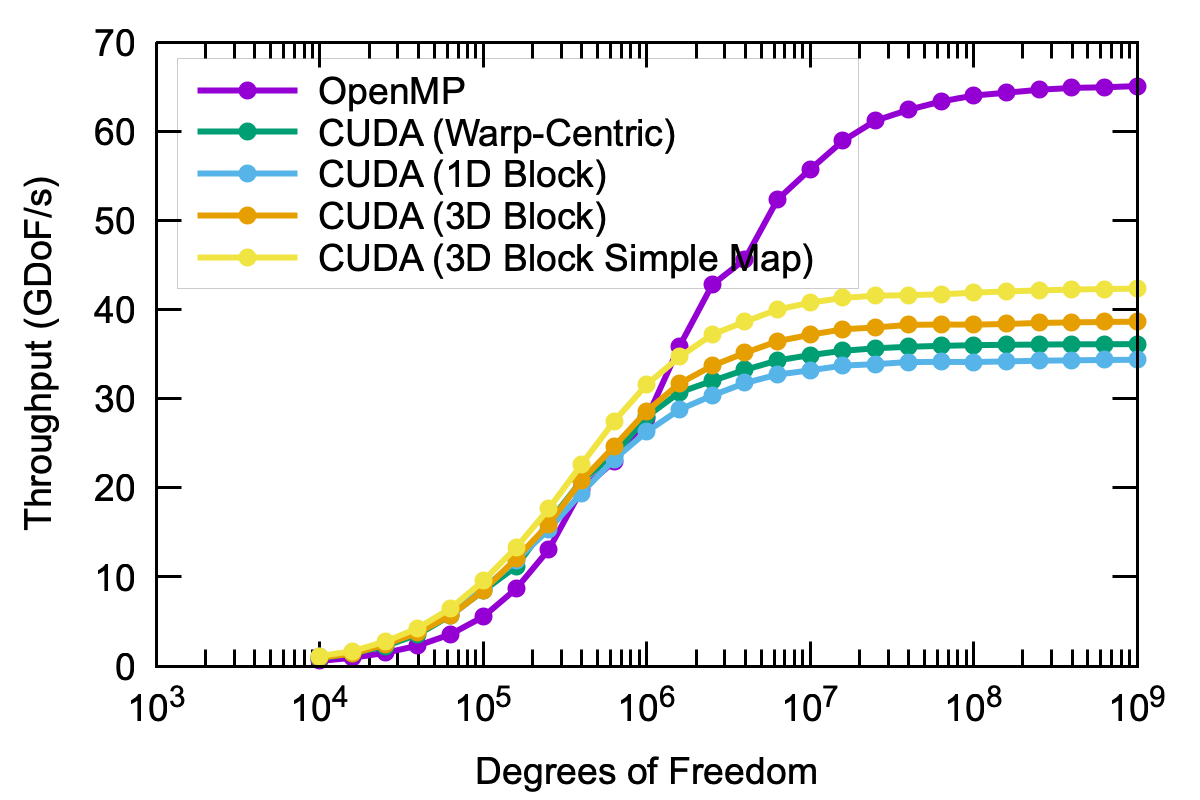
\includegraphics[width=0.8\textwidth]{gh200_templated} % replace with your filename
  \caption{BK1 performance for templated kernel, $q = 4$, Nvidia GH200 (Hopper).}
  \label{fig:gh200_templated}
\end{figure}

\begin{figure}[htbp]
  \centering
  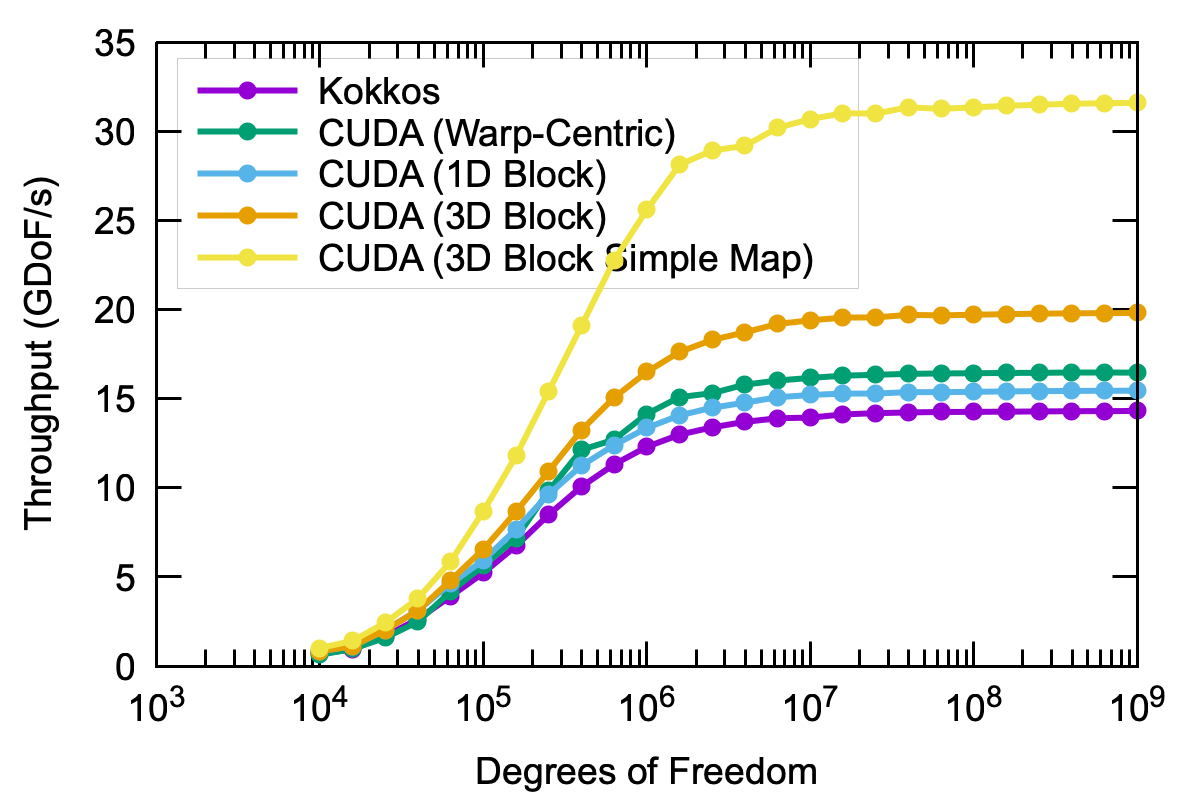
\includegraphics[width=0.8\textwidth]{gh200_variable} % replace with your filename
  \caption{BK1 performance for variable kernel, $q = 4$, Nvidia GH200 (Hopper).}
  \label{fig:gh200_variable}
\end{figure}


\subsection{OpenCL}

For experimentation across a wider array of potential accelerator devices, the CUDA kernels have also been translated to the OpenCL-C language for use with the vendor-neutral OpenCL framework from Khronos.
OpenCL remains widely supported across both CPU and GPU devices from multiple vendors.
The verbose setup required via the OpenCL runtime API, the split kernel source model, and restriction to C level language semantics, are some of the main criticisms from scientific software developers. 
The growing popularity of C++ coupled with powerful syntactic features has shifted the attention to more expressive programming models including SYCL and Kokkos, which provide similar capabilities as OpenCL, but are arguably simpler to use. 

\begin{figure}[htbp]
  \centering
  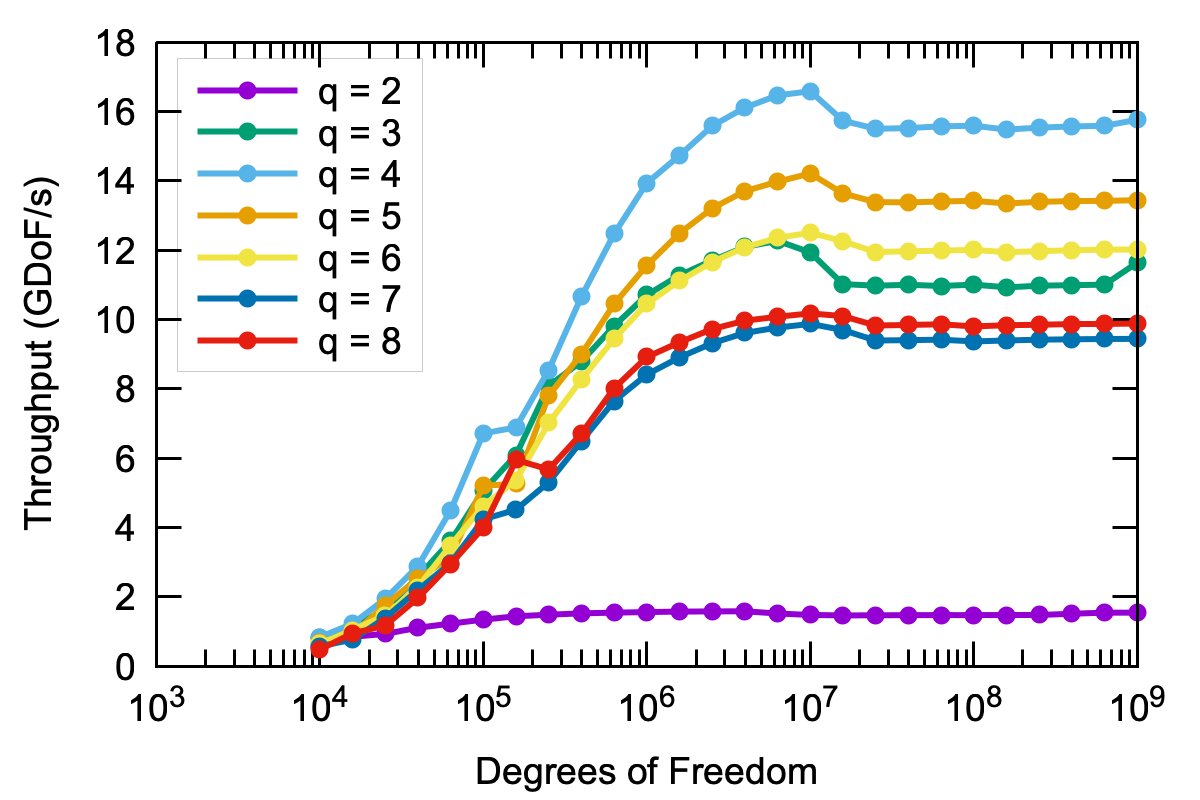
\includegraphics[width=0.8\textwidth]{pvc_opencl} % replace with your filename
  \caption{BK1 using OpenCL and 3D Simple Map work-item strategy, Intel Max Series 1550 GPU (Ponte Vecchio).}
  \label{fig:pvc_opencl}
\end{figure}

\begin{figure}[htbp]
  \centering
  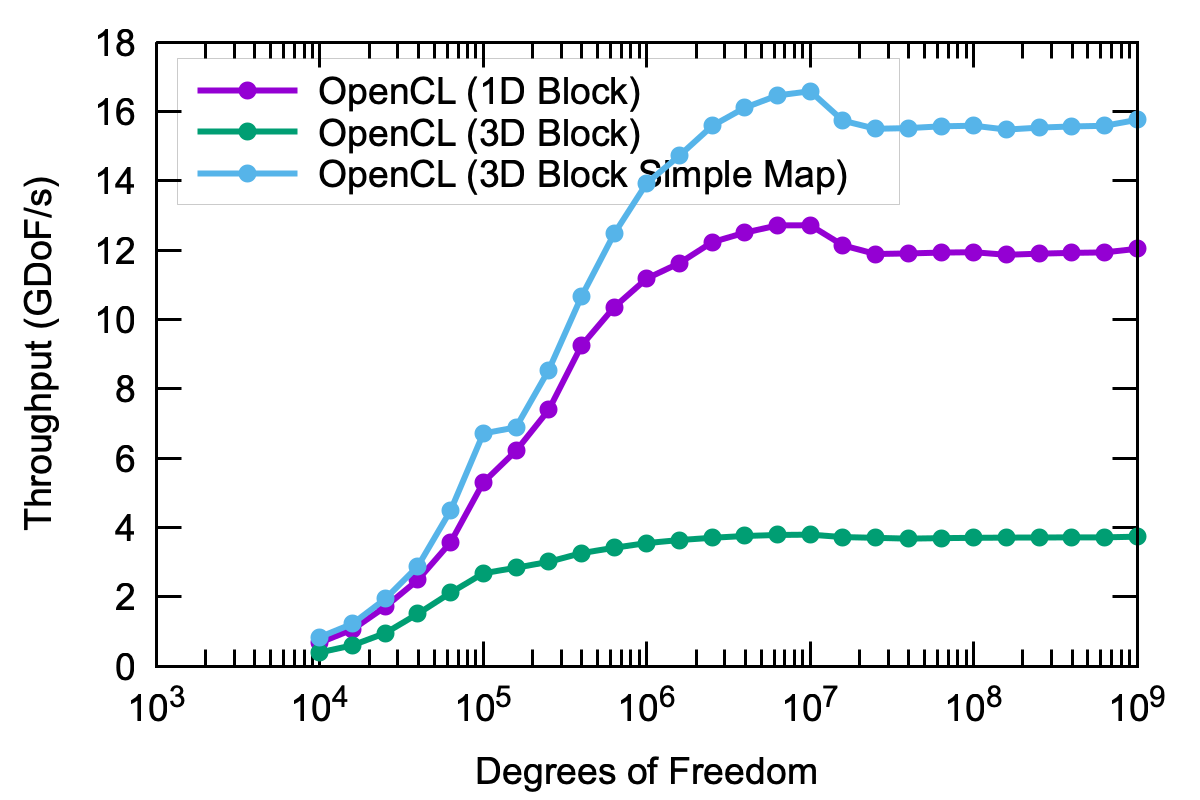
\includegraphics[width=0.8\textwidth]{pvc_opencl_q4_static} % replace with your filename
  \caption{BK1 performance for templated kernel, $q = 4$, Intel Max Series 1550 GPU (Ponte Vecchio).}
  \label{fig:pvc_static}
\end{figure}

\begin{figure}[htbp]
  \centering
  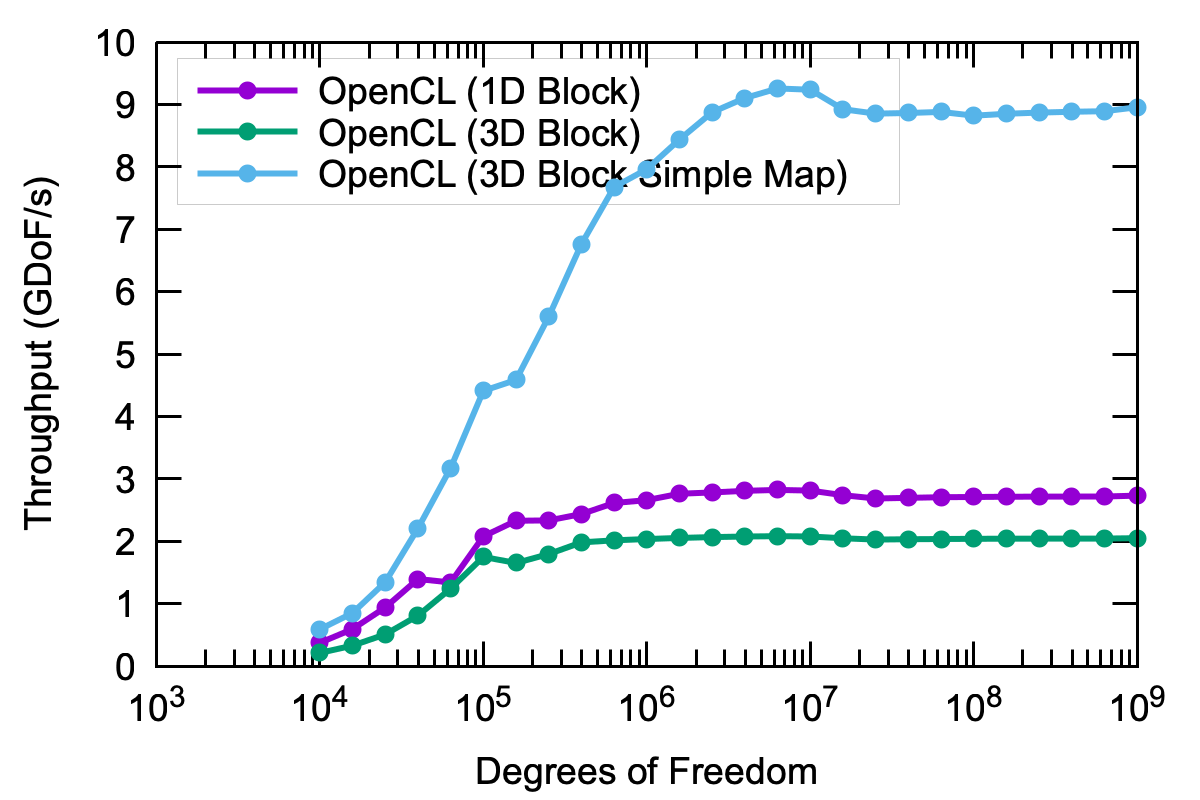
\includegraphics[width=0.8\textwidth]{pvc_opencl_q4_dynamic} % replace with your filename
  \caption{BK1 performance for variable kernel, $q = 4$, Intel Max Series 1550 GPU (Ponte Vecchio).}
  \label{fig:pvc_dynamic}
\end{figure}

\subsection{OpenMP Offloading}

Since its introduction in OpenMP 4.5, offloading has become an integral component
of this directive-based parallel programming framework.
Adding OpenMP directives for offloading to an existing code can be quite straightforward,
assuming the right data structures and loop patterns are already in place.
When using OpenMP for GPU offloading, it is important to distinguish between two
categories of directives for memory movement and work sharing.

Similar to other GPU programming models, OpenMP offers fine-grained control over the hierarchical parallelism in terms of teams and threads. These are reflected by the two directives, `omp teams' which replicates execution across a league of teams and `omp parallel' which replicates execution across threads of a team. 
The two directives can also be used to program in a SPMD-like mode (also called ``me'' mode). 
Typically however, the directives are combined with work-sharing
constructs like `distribute' and `for' which control the parallelization of (nested) loops.
A very useful work-sharing construct is the `[teams] loop` directive, which provides 
a descriptive form of parallelism in contrast to other prescriptive directives.
With the `target [teams] loop' directive, the precise distribution of the loop iteration space across teams and threads is left to the compiler. 
As explained by \cite{Deakin23}, this kind of descriptiveness can provide
superior performance portability, assuming the compiler succeeds to auto-parallelize
the loop well.

\begin{lstlisting}[language=C++,caption={The `omp teams loop' directive},
                   label={lst:omp_loop}]
#pragma omp target \
    map(to: basis0[:nm0*nq0], basis1[:nm1*nq1], basis2[:nm2*nq2]) \
    map(to: in[:nelmt*nm0*nm1*nm2], JxW[:nelmt*nq0*nq1*nq2]) \
    map(from: out[:nelmt*nm0*nm1*nm2])
#pragma omp teams loop
for(size_t e = 0; e < nelmt; ++e) {
    /* ... sum factorization ... */
}
\end{lstlisting}

Listing \ref{lst:omp_loop} shows an excerpt of from the BK1 algorithm, parallelized using using the \texttt{omp teams loop} directive. 
The loop shown here is the outer loop across elements of the E-vector in CEED terminology.
First a `target' region is opened, instructing the compiler to generate
device code for the scope of the upcoming for-loop. 
The `map' clauses are used to communicate the array sizes and exert control over the direction of memory movement to the minimum necessary.
Finally, the `teams loop` directive is used to divide the calculation of elements across threads in a concurrent fashin.
For this particular kernel the simpler `omp loop' directive (without `teams`) would also be sufficient, but instead we wanted to emphasize the assigment of elements across teams first.

\begin{figure}[htbp]
  \centering
  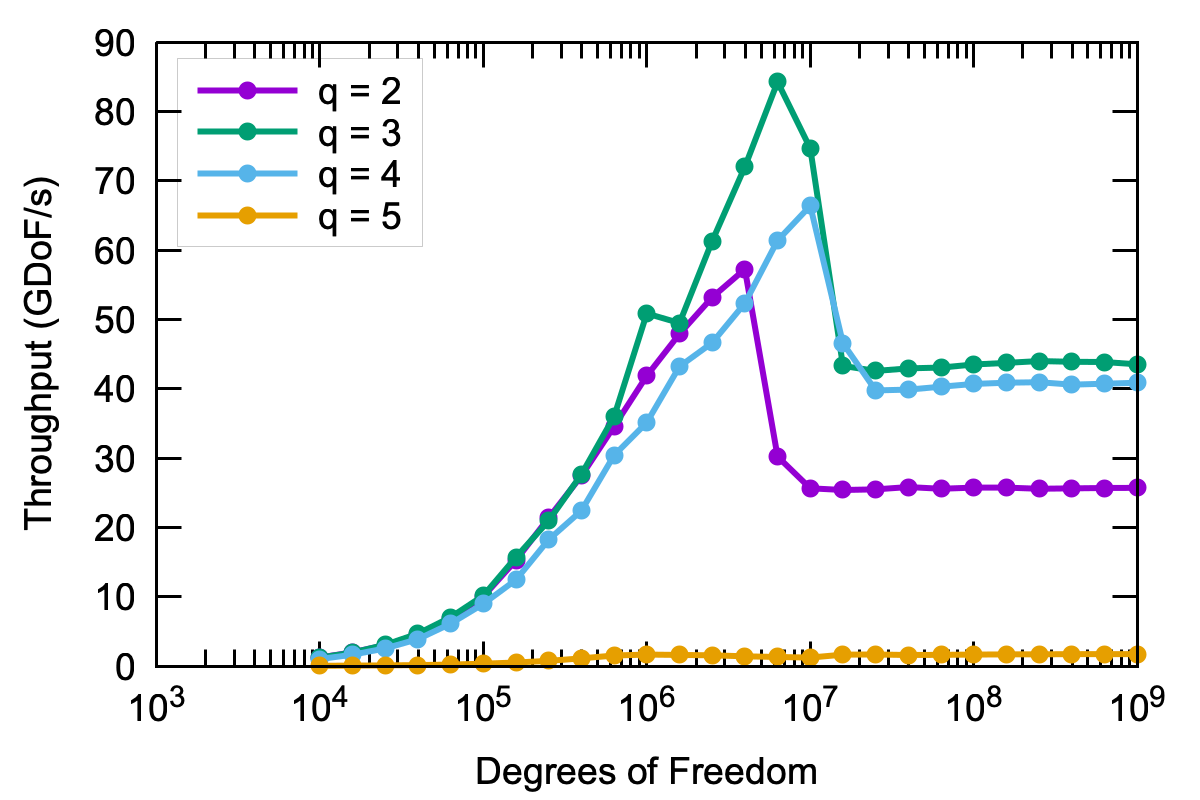
\includegraphics[width=0.8\textwidth]{pvc_openmp} % replace with your filename
  \caption{BK1 using OpenMP, Intel Max Series 1550 GPU (Ponte Vecchio).}
  \label{fig:pvc_openmp}
\end{figure}


\subsection{Tiny Tensor Compiler}

\label{sec:tinytc}

The Tiny Tensor Compiler (TinyTC) is an open-source tensor compiler developed by Intel for efficient execution of tensor computations on CPUs and GPUs. TinyTC compiles programs written in a domain-specific tensor language into OpenCL-C or SPIR-V, supporting runtime environments such as OpenCL, Level Zero, and SYCL. C and C++ APIs are available. TinyTC assumes a batched execution model, where each kernel is executed by a work-group with concurrent work-items, and the compiler maps tensor operations to efficient GPU instructions, including cooperative GEMMs and subgroup vectorization. Further details of the execution model and available instructions can be found in the online documentation.\footnote{\url{https://intel.github.io/tiny-tensor-compiler/manual/tensor-ir.html}, accessed on 25/08/2028}

Domain-specific languages (DSLs) provide abstraction and performance portability by expressing operations in a form closer to the mathematical problem rather than low-level loops. In recent years, DSLs such as FreeFem++ or FEniCS UML allow variational forms to be compiled into optimized C or LLVM IR. Similarly, TinyTC aims to represent tensor operations, representing multi-dimensional contractions, fusions, and GEMMs in a dedicated tensor language, but remains unaware of finite element specifics.

Our first test of TinyTC aims to accelerate the finite element mass matrix evaluation (BK1) using sum factorization. As a first demonstration of tensor language we present the BK1 kernel using an algorithm presented by \cite{Swirydowicz19}, see Listing \ref{lst:tinytc}, where each tensor product is implemented using the loop over GEMM approach. For simplicity the implementation uses four temporary arrays, \texttt{wsp0}-\texttt{wsp4}, allocated in group local storage.

\begin{lstlisting}[language=TensorIR,caption={BK1 using Tensor IR},basicstyle=\ttfamily\tiny,
                   label={lst:tinytc}]
func @sum_factorization(%basis0: memref<f32x3x4>,
                        %basis1: memref<f32x3x4>,
                        %basis2: memref<f32x3x4>,
                        %JxW:    memref<f32x4x4x4x?>,
                        %in:     memref<f32x3x3x3x?>,
                        %out:    memref<f32x3x3x3x?>) {

    %gid = group_id

    %wsp0 = alloca -> memref<f32x3x3x3>; // Reserve temporary memory
    %wsp1 = alloca -> memref<f32x3x3x4>; // Reserve temporary memory
    %wsp2 = alloca -> memref<f32x3x4x4>; // Reserve temporary memory
    %wsp3 = alloca -> memref<f32x4x4x4>; // Reserve temporary memory
    %wsp4 = alloca -> memref<f32x4x4x4>;

    %J_e = subview %JxW[:,:,:,%gid] : memref<f32x4x4x4x?>;
    %in_e = subview %in[:,:,:,%gid] : memref<f32x3x3x3x?>;
    %out_e = subview %out[:,:,:,%gid] : memref<f32x3x3x3x?>;

    for %j1 = 0, 3 { ; Batch of GEMMs
        %tmp = subview %in_e[:,%j1,:] : memref<f32x3x3x3>
        %res = subview %wsp1[:,%j1,:] : memref<f32x3x3x4>
        gemm.n.n 1.0, %tmp, %basis0, 0.0, %res :
            f32, memref<f32x3x3,strided<1,9>>, memref<f32x3x4>, f32, memref<f32x3x4,strided<1,9>>;
    }

    for %j2 = 0, 4 { ; Batch of GEMMs
        %tmp = subview %wsp1[:,:,%j2] : memref<f32x3x3x4>
        %res = subview %wsp2[:,%j2,:] : memref<f32x3x4x4>
        gemm.n.n 1.0, %tmp, %basis1, 0.0, %res :
            f32, memref<f32x3x3>, memref<f32x3x4>, f32, memref<f32x3x4,strided<1,12>>
    }

    for %j3 = 0, 4 { ; Batch of GEMV
        for %p3 = 0, 4 {
            %tmp = subview %wsp2[:,%p3,%j3] : memref<f32x3x4x4>
            %res = subview %wsp3[:,%j3,%p3] : memref<f32x4x4x4>
            gemv.t 1.0, %basis2, %tmp, 0.0, %res :
                f32, memref<f32x3x4>, memref<f32x3>, f32, memref<f32x4> 
        }
    }    

    %flat1 = fuse %J_e[0,2] : memref<f32x4x4x4>
    %flat2 = fuse %wsp3[0,2] : memref<f32x4x4x4>
    %flat3 = fuse %wsp4[0,2] : memref<f32x4x4x4>

    hadamard 1.0, %flat1, %flat2, 0.0, %flat3 :
        f32, memref<f32x64>, memref<f32x64>, f32, memref<f32x64>

    for %q6 = 0, 4 {                               ; Step 6
        for %p6 = 0, 4 {
            %tmp = subview %wsp4[:,%q6,%p6] : memref<f32x4x4x4>
            %res = subview %wsp2[:,%p6,%q6] : memref<f32x3x4x4>
            gemv.n 1.0, %basis2, %tmp, 0.0, %res :
                f32, memref<f32x3x4>, memref<f32x4>, f32, memref<f32x3> 
        }
    }

    for %p7 = 0, 4 {
        %tmp = subview %wsp2[:,%p7,:] : memref<f32x3x4x4>
        %res = subview %wsp1[:,:,%p7] : memref<f32x3x3x4>
        gemm.n.t 1.0, %tmp, %basis1, 0.0, %res :
            f32, memref<f32x3x4,strided<1,12>>,memref<f32x3x4>, f32, memref<f32x3x3>
    }

    for %j8 = 0, 3 {
        %tmp = subview %wsp1[:,%j8,:] : memref<f32x3x3x4>
        %res = subview %out_e[:,%j8,:] : memref<f32x3x3x3>
        gemm.n.t 1.0, %tmp, %basis0, 0.0, %res :
            f32, memref<f32x3x4,strided<1,9>>, memref<f32x3x4>, f32, memref<f32x3x3,strided<1,9>>
    }
    
}
\end{lstlisting}

As the \texttt{alloca} instruction reserves temporary memory in shared local memory, TinyTC automatically inserts thread barriers between each of the six GEMM passes to ensure functional correctness. 
The kernel shown above achieved 10 GDoF/s on the Intel Ponte Vecchio GPU, roughly one quarter of the performance we observed using OpenMP. 
One of several optimizations possible is fusing dimensions, to obtain larger GEMMs with a more favourable operation count. 
For instance in step 1 (the \texttt{j1}-loop), the loop over GEMMs can be rewritten as a single GEMM by fusing dimensions (Listing \ref{lst:tinytc_fuse}).

\begin{lstlisting}[language=TensorIR,caption={BK1 using Tensor IR},basicstyle=\ttfamily\small,
                   label={lst:tinytc_fuse}]
    %tmp1 = fuse %in_e[0,1] : memref<f32x9x3>
    %res1 = fuse %wsp1[0,1] : memref<f32x9x4,local>    
    gemm.n.n %c1, %tmp1, %basis0, %c0, %res1
\end{lstlisting}

Other GEMM steps can be fused in a similar manner, however this only delivered a few percent improvement. Upon consultation with the TinyTC author it became apparent a different strategy would be needed to obtain performant execution and optimal SIMD utilization of the PVC architecture.
In collaboration with Intel, we are currently investigating the application of index fusion, batch vectorization and memory layout transformations to guarantee optimal register and SIMD usage.

Despite these initial challenges, the use of a specialized tensor DSL offers numerous potential benefits including,
\begin{itemize}
\item Readability and maintenance: kernels are expressed in a high-level tensor operations rather than nested loops
\item Hardware portability: TinyTC maps tensor operations to different architectures without rewriting kernels. Currently, this is portability is limited to Intel devices.
\item Runtime specialization: kernels written in IR are ingested as strings for just-in-time compilation, allowing constant loop bounds for optimal looping and GEMM optimizations
\item Optimized memory and SIMD usage: temporary arrays are automatically placed in shared local memory; cooperative matrix instructions can reduce synchronization overhead.
\end{itemize}


\section{Streaming Kernels}

Iterative linear system solvers make heavy use of low arithmetic intensity operations, so called streaming operations.
When matrix-free high-order FEM schemes are combined with iterative solvers. 
As shown previously by Kronbichler et al. \cite{kronbichler2023enhancing} on the case of the conjugate gradient method, above a certain problem size the streaming operations contribute a significant chunk of the run-time.

In this section we present some preliminary results on the performance and portability of
streaming operations implemented using different frameworks on CPU and GPU architectures.

% FIXME


\section{Energy Efficiency}

The shift to heterogeneous computing with accelerators is driven not only by the demand for higher performance but also by the increasing power and thermal constraints of modern semiconductor technology. These pressures have led to hardware specialization for more energy-efficient computing, as reflected in the Green500 list, where GPU-accelerated systems dominate. As shown by Cielo et al. \cite{Cielo2025} in a case study of an astrophysical simulation, accelerators can deliver a 5–10× improvement in energy efficiency (flops per watt) over CPUs. This advantage stems from their throughput-oriented parallel design, which contrasts with the latency-focused nature of traditional CPUs.

Maximizing these benefits requires energy-aware practices from both HPC practitioners and application developers. Since power and energy usage vary across devices, workloads, and runtime conditions, precise modeling is difficult, making empirical measurement essential. System-level monitoring frameworks such as Intel’s RAPL, AMD uProf, NVIDIA’s NVML, or Arm’s Streamline provide access to hardware counters, while job- and process-level tools such as the Energy Aware Runtime, perf, likwid-powermeter, and PAPI enable finer-grained insights. For kernel-level breakdowns, vendor tools like NVIDIA Nsight or Intel VTune are available, but they often involve heavy instrumentation and vendor lock-in. In practice, lightweight and portable solutions remain highly attractive.

To this end, Cielo et al. \cite{Cielo2025} proposed a process-based approach in which applications call an external ``energy-meter'' script during execution. The script samples instantaneous power through utilities such as `nvidia-smi', `xpu-smi', or `perf', and integrates the readings to estimate total energy consumption. A key advantage is that programmers can call the meter only around the sections of interest, thereby excluding initialization or I/O phases and focusing on the algorithmic kernels. The method is portable, simple to maintain, and adaptable to a variety of devices or custom meters. 

In the remaining period of this work package, we plan to adopt this strategy to measure the energy usage of the core algorithmic kernels and gain an overview of their power behavior. Although we have not yet carried out such experiments, we take inspiration from a recent presentation by S. Cielo (LRZ), who demonstrated the benefits of these techniques, and we intend to implement them as part of our future performance and energy-efficiency evaluations.

\section{Algorithmic development}


\section{Next steps}

\begin{itemize}
    \item TinyTC kernel optimization using fusion and cross-element vectoritation
    \item Use of advanced multigrid solvers and preconditioners
\end{itemize}


\section{Hardware systems}

\begin{center}
    \begin{table}[h!]
    \small
    \caption{GPUs used for evaluation}
    \renewcommand{\arraystretch}{1.25}
    \label{tab:example_table}
    \begin{tabular}{|l|l|l|c|}
    \hline
    \textbf{Column 1} & \textbf{Ampere} & \textbf{Hopper} & \textbf{Ponte Vecchio} \\
    \hline
    execution units & Description & Category & Value \\
    base frequency & Description & Category & Value \\
    SIMT/SIMD width & Description & Category & Value \\
    last level cache & Description & Category & Value \\
    memory bandwidth & Description & Category & Value \\
    \hline
    \end{tabular}
    \end{table}
\end{center}

\bibliographystyle{plainnat}
\bibliography{refs}        % refs.bib in the same folder


\end{document}
